\section{Refinando petr\'oleo}
\subsection{Descripci\'on de la problem\'atica}
\subsection{Resoluci\'on propuesta y justificaci\'on}
\subsection{An\'alisis de la complejidad}
	El algoritmo recibe por par\'ametro un grafo no dirigido en forma de cantidad de nodos (numerados arbitrariamente de 0 a n-1) y los ejes que existen entre cada par de nodos, y el costo de construir una refiner\'ia. Es importante destacar que la cantidad de ejes est\'a acotada por $O(n^2)$, porque cada nodo, en el peor caso, puede conectarse con todos los nodos del grafo, excepto consigo mismo, es decir que para cada nodo, existen a lo sumo n-1 ejes que entran y salen del mismo. Tomamos como notaci\'on $n = cantNodos$ y $m = cantEjes$.
	
	Lo primero que hace es identificar los ejes donde es conveniente colocar una tuber\'ia para conectar dos pozos en vez de construir una refiner\'ia sobre ambos, aplicando el algoritmo de $Kruskal$, apoyados sobre la estructura $Union-Find$.
	
	Este paso ordena los ejes mediante sort \textcolor{red}{Poner referencia a sort si todavia no se uso} de la librer\'ia standar de $C$. Esto tarda $O(m.log(m))$, lo que es lo mismo que $O(n^2.log(n^2))$, que por propiedades del logaritmo es $O(n^2.2.log(n))$, eliminando constantes es $O(n^2.log(n))$. Luego por cada eje de ejes, si no forma un ciclo dentro de la componente conexa a la que pertenece, une ambos pozos, pero solo lo agrega al resultado si cuesta menos que poner una refiner\'ia. Este paso aprovecha la estructura de conjuntos disjuntos $Union-Find$, para ver si dos conjuntos son dijuntos y eventualmente unirlos "r\'apidamente". Dado que lo implementamos con las heur\'isticas de $path compression$ y $union by rank$, la complejidad de $m$ operaciones find_set y union-set m\'as una llamada a make_set de complejidad $O(n)$, ejecutan en tiempo $O(m\alpha(n))$, donde $\alpha(n)$ es la inversa de funci\'on de Ackerman:
	
	A(m,n) = 2\uparrow 

\subsection{C\'odigo fuente}

	\begin{codesnippet}
	\begin{verbatim}
    class UnionFind {
    public:
        	UnionFind(int tamano);
        ~UnionFind();
        int find_set(int x);
        void union_set(int x, int y);
        bool is_in(int x, int y);

    private:
        vector<int> parent;
        vector<int> rank;
    };
	\end{verbatim}
	\end{codesnippet}

	\begin{codesnippet}
	\begin{verbatim}
    	UnionFind::UnionFind(int tamano){
        	parent = vector<int>(tamano);
        rank = vector<int>(tamano);
    //cada indice es su propio representante, su ranking es 0
        for (int i = 0; i < tamano; ++i) {
            parent[i] = i;
            rank[i] = 0;
        }
    }
	\end{verbatim}
	\end{codesnippet}

	\begin{codesnippet}
	\begin{verbatim}
    int UnionFind::find_set(int x) {
    //si es representante lo devuelvo, si no lo hago apuntar directamente al representante
    //para que llamadas consecutivas cuesten tiempo constante
        if(parent[x] != x)
            parent[x] = find_set(parent[x]);
        return parent[x];
    }
	\end{verbatim}
	\end{codesnippet}

	\begin{codesnippet}
	\begin{verbatim}
    void UnionFind::union_set(int x, int y) {
    //buscamos representantes de ambos elementos
    //requiere que no esten en el mismo conjunto
        int rx = find_set(x);
        int ry = find_set(y);
    //incluyo el de menor ranking en el de mayor para mantener balanceada la estructura
        if(rank[rx] < rank[ry]){
            parent[rx] = ry;
        }
        else{
            parent[ry] = rx;
            if(rank[ry] == rank[rx])
                rank[rx]++;
        }
    }
	\end{verbatim}
	\end{codesnippet}

	\begin{codesnippet}
	\begin{verbatim}
    bool UnionFind::is_in(int x, int y) {
        return find_set(x) == find_set(y);
    }
	\end{verbatim}
	\end{codesnippet}

	\begin{codesnippet}
	\begin{verbatim}
    struct eje {
        unsigned int pozoA;
        unsigned int pozoB;
        unsigned int costoTuberia;
        bool operator< (const eje& otro) const{
            return costoTuberia < otro.costoTuberia;
        }
    };
	\end{verbatim}
	\end{codesnippet}

	\begin{codesnippet}
	\begin{verbatim}
    int main(int argc, char const *argv[]){
        unsigned int pozos, cantConexiones, costoRefineria;
        unsigned int pozoA, pozoB, costoTuberia;
        cin >> pozos >> cantConexiones >> costoRefineria;
        vector<eje> ejes;
    //leemos la entrada, la almacenamos en ejes
        for (int i = 0; i < cantConexiones; ++i){
            cin >> pozoA >> pozoB >> costoTuberia;
            pozoA--;
            pozoB--;
            eje conex;
            conex.pozoA = pozoA;
            conex.pozoB = pozoB;
            conex.costoTuberia = costoTuberia;
            ejes.push_back(conex);
        }
    //aplicamos el algoritmo
        refinandoPetroleo(ejes, pozos, costoRefineria);
        return 0;
    }
	\end{verbatim}
	\end{codesnippet}

	\begin{codesnippet}
	\begin{verbatim}
    int refinandoPetroleo(vector<eje>& ejes, int cantPozos, int costoRefineria){
    //generamos los arboles minimos para cada componente conexa, en realidad solo los ejes que cuesten menos que poner refinerias
        vector<eje> conexionesMinimas = generarArbolesMinimos(ejes, costoRefineria, cantPozos);
        UnionFind conexos(cantPozos);
        int costoTotal = 0, cantRef = 0;
    //armamos un union-find para identificar componentes triviales, en las demas solo hara falta poner una refineria
    //en el representante de la componente pues los tubos son mas baratos para unir los distintos pozos
        for (int i = 0; i < conexionesMinimas.size(); ++i) {
            conexos.union_set(conexionesMinimas[i].pozoA, conexionesMinimas[i].pozoB);
            costoTotal += conexionesMinimas[i].costoTuberia;
        }
    //en las componentes triviales van refinerias
        vector<bool> refinerias(cantPozos);
        for (int i = 0; i < cantPozos; ++i) {
            if(conexos.find_set(i) == i){
                refinerias[i] = true;
                costoTotal += costoRefineria;
                cantRef += 1;
            }
        }
    //cout pedido
        cout << costoTotal << " " << cantRef << " " << conexionesMinimas.size() << endl;
        for (int i = 0; i < refinerias.size(); ++i) {
            if(refinerias[i])
                cout << i+1 << " ";
            }
        cout << endl;
        for (int i = 0; i < conexionesMinimas.size(); ++i) {
            cout << conexionesMinimas[i].pozoA+1 << " " << conexionesMinimas[i].pozoB+1 << endl;
        }
        return costoTotal;
    }
	\end{verbatim}
	\end{codesnippet}

	\begin{codesnippet}
	\begin{verbatim}
    vector<eje> generarArbolesMinimos(vector<eje>& ejes, int costoRefineria, int cantPozos){
        UnionFind bosqueMinimo(cantPozos);
        vector<eje> res;
    //ordenamos los ejes segun su costo para obtener en tiempo constante, los menores
        sort(ejes.begin(), ejes.end());
        for (int i = 0; i < ejes.size(); ++i) {
    //si agregar el eje no forma ciclo
        if(!bosqueMinimo.is_in(ejes[i].pozoA,ejes[i].pozoB)){
    //lo uno y si cuesta menos que poner una refineria, lo agrego a res
            bosqueMinimo.union_set(ejes[i].pozoA, ejes[i].pozoB);
                if(ejes[i].costoTuberia < costoRefineria){
                    eje conex;
                    conex.pozoA = ejes[i].pozoA;
                    conex.pozoB = ejes[i].pozoB;
                    conex.costoTuberia = ejes[i].costoTuberia;
                    res.push_back(conex);
                }
            }
        }
        return res;
    }
	\end{verbatim}
	\end{codesnippet}

\subsection{Experimentaci\'on}
\subsubsection{Constrastaci\'on Emp\'irica de la complejidad}
	Para llevar a cabo esta experimentaci\'on, consideramos el peor caso posible de cantidad de ejes del grafo, es decir que habr\'a exactamente $n.(n-1)$ ejes (cada nodo puede conectarse con cualquier nodo del grafo, excepto consigo mismo), variando la cantidad de nodos.
	
	Los tiempos de ejecuci\'on para cada n (cantidad de nodos) fueron los siguientes:
	
	\begin{table}[htb]
	\centering
	\begin{tabular}[c]{|l|l|}

		\hline
n & Tiempo en segundos\\
		\hline
50	&	0.0005254864\\
		\hline
100	&	0.002332719\\
		\hline
150	&	0.0059328642\\
		\hline
200	&	0.01065945\\
		\hline
250	&	0.0178728144\\
		\hline
300	&	0.0277215188\\
		\hline
350	&	0.0373807766\\
		\hline
400	&	0.0487278266\\
		\hline
450	&	0.0661190683\\
		\hline
500	&	0.0807527896\\
		\hline
550	&	0.0978193478\\
		\hline
600	&	0.126140013\\
		\hline
650	&	0.146378511\\
		\hline
700	&	0.168847877\\
		\hline
750	&	0.192539493\\
		\hline
800	&	0.219705288\\
		\hline
850	&	0.267457097\\
		\hline
900	&	0.301437881\\
		\hline
950	&	0.332602623\\
		\hline
1000	&	0.366929358\\
		\hline
		
	\end{tabular}
	%\caption{Tabla muy sencilla.}
	%\label{tabla:n.png}
	\end{table}

  \begin{figure}[h!]
   \begin{center}
 	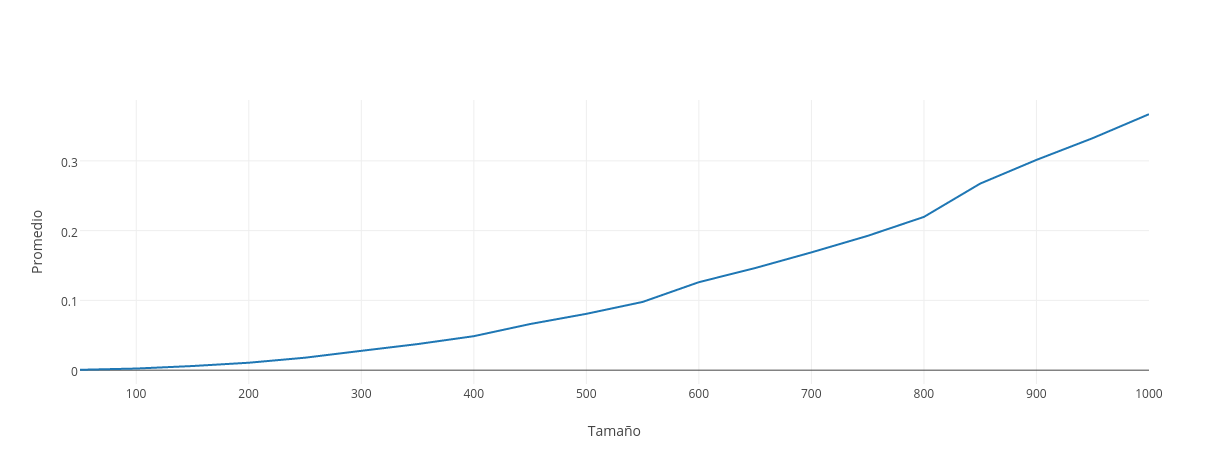
\includegraphics[scale=0.4]{imagenes/ej3/n2logn.png}
% 	\caption{}
% 	\label{n.png}
   \end{center}
 \end{figure}
 \newpage

Dado que la Cota de Complejidad planteada te\'oricamente es de $O(n^2.log(n))$, era esperable que la curva sea una par\'abola creciente.

A simple vista, no se puede apreciar si la relaci\'on que tienen respecto de tama\~no/tiempo es efectivamente la que buscamos (pues casi todas las curvas polinomiales tienen gr\'aficos similares). Por este motivo, como siguiente paso decidimos comenzar a linealizar los tiempos, dividiendo a cada uno por $log(n)$.

   \begin{figure}[h!]
   \begin{center}
 	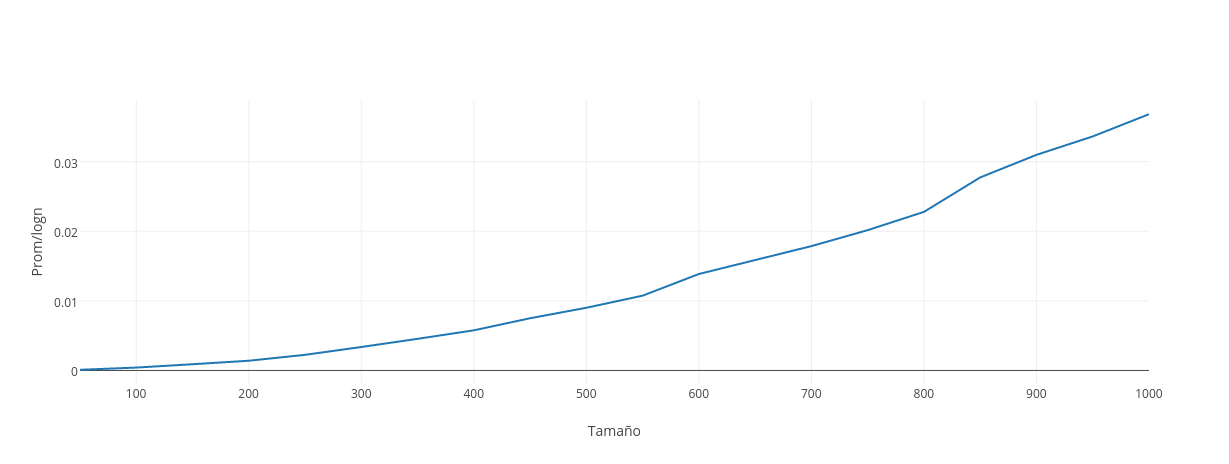
\includegraphics[scale=0.4]{imagenes/ej3/n2.png}
% 	\caption{}
% 	\label{caballito}	
   \end{center}
 \end{figure}
 \newpage

	La morfolog\'ia de este gr\'afico es similar a la anterior, sigue siendo una par\'abola creciente, por lo tanto terminaremos de linealizar, dividiendo a cada uno por $n$, para ver si se trata de la par\'abola cuadr\'atica.\\

   \begin{figure}[h!]
   \begin{center}
 	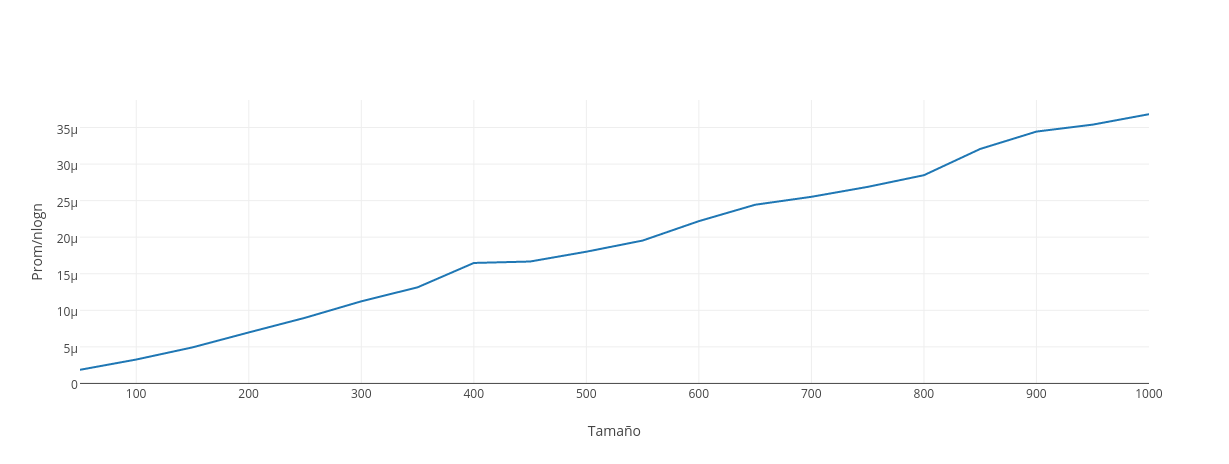
\includegraphics[scale=0.4]{imagenes/ej3/n.png}
% 	\caption{}
% 	\label{caballito}	
   \end{center}
 \end{figure}
 \newpage

	Efectivamente puede observarse que el comportamiento es lineal. Por lo tanto, podemos afirmar que nuestra experimentaci\'on condice a la Cota Te\'orica planteada de $O(n^2.log(n))$.